\documentclass[tikz]{standalone}
\usetikzlibrary{scopes}
%\'{a}\^{g} ki di-ta nu-\^{g}en-\'{a}\^{g} ki --eme-gir$_\text{7}$ qa-b\^{u}m
%You are not one who stays in one place, you are one who is everywhere. --Sumerian Saying

\tikzset{
    wedge/.pic={
        \filldraw (0,2) -- (1.5,3.5) .. controls (0.8,2.2) and (1.4, 1) .. (2.25,0) -- cycle;
    },
    stick/.pic={
        \filldraw (0,5) .. controls (0.9,4) .. (1,0) .. controls (1.1,4.2) .. (2,5) .. controls (0.9,4.7) .. (0,5);
    },
    fatstick/.pic={
        \filldraw (0,5) .. controls (0.9,4) .. (1,3) .. controls (1.1,4.2) .. (2,5) .. controls (0.9,4.7) .. (0,5);
    }
}

\begin{document}
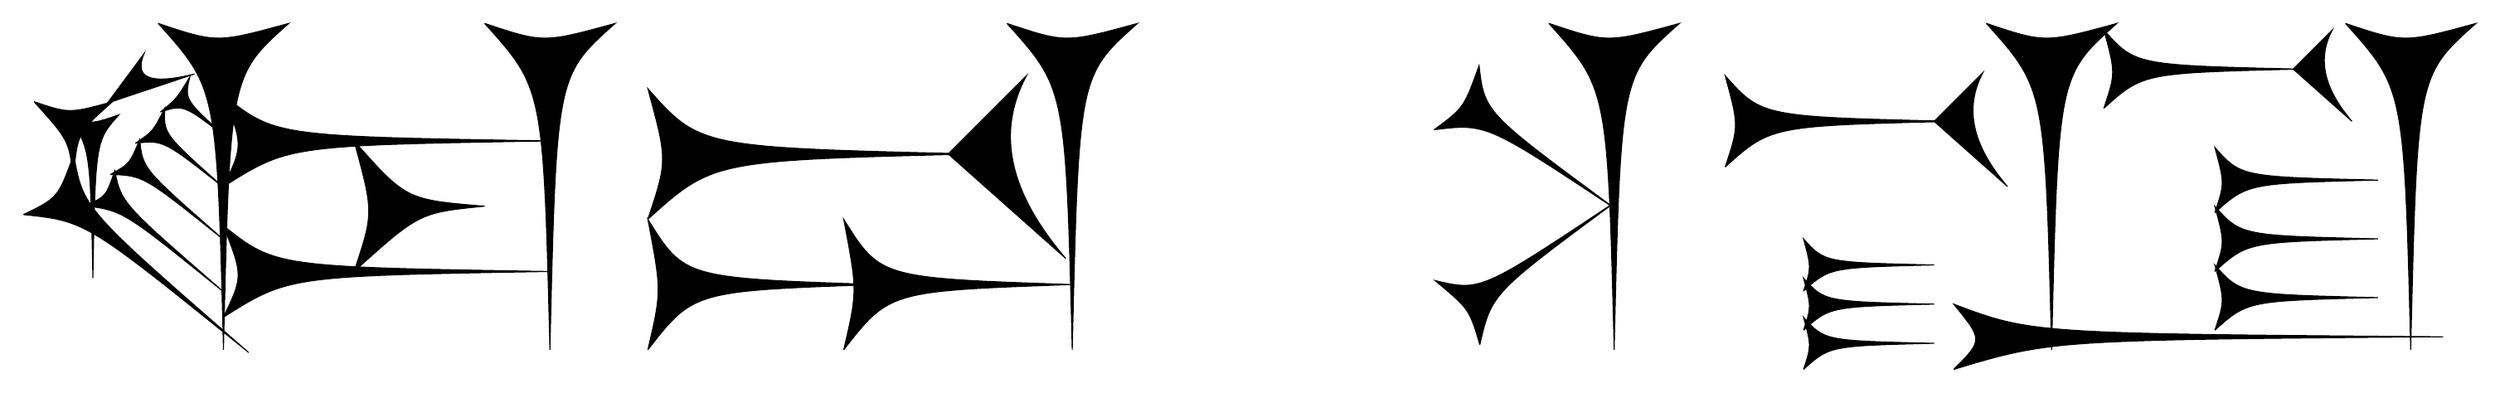
\begin{tikzpicture}
    %eme
    { [black]
    \pic at (0,0) {stick};
    \pic at (5,0) {stick};
    \pic at (6,0.5) [rotate=90, xscale=0.7] {stick};
    \pic at (6,2.5) [rotate=90, xscale=0.7] {stick};
    \pic at (8,1.2) [rotate=90] {fatstick};
    \pic at (1,-0.5) [rotate=50, xscale=0.6, yscale=0.8] {stick};
    \pic at (-1.9,0.8) [scale=0.6] {fatstick};
    \pic at (-1.4,1.1) [xscale=0.4,yscale=0.5] {stick};
    \pic at (0.8,0.6) [rotate=50, xscale=0.35,yscale=0.5] {stick};
    \pic at (0.8,1.4) [rotate=50, xscale=0.35,yscale=0.4] {stick};
    \pic at (0.8,2.2) [rotate=50, xscale=0.35,yscale=0.3] {stick};
    \pic at (0.8,3) [rotate=50, xscale=0.35,yscale=0.2] {stick};
    \pic at (-0.55,3.45) [rotate=35, xscale=0.6, yscale=0.2] {wedge};
    }
    %gir$_\text{7}$
    { [xshift=11cm]
    \pic at (0,0) [rotate=90, yscale=0.7] {stick};
    \pic at (3,0) [rotate=90, yscale=0.7] {stick};
    \pic at (1.5,2) [rotate=90] {stick};
    \pic at (1.1,1.4) [scale=0.8] {wedge};
    \pic at (2,0) {stick};
    }
    %qu
    { [xshift=22cm]
    \pic at (0,1.65) [rotate=55, scale=0.6] {stick};
    \pic at (0.7,1.8) [rotate=125, scale=0.6] {stick};
    \pic at (-0.7,0) {stick};
    }
    %b\^{u}m
    { [xshift=28cm]
    \pic at (-0.8,-0.3) [rotate=90, scale=0.4] {stick};
    \pic at (-0.8,0.3) [rotate=90, scale=0.4] {stick};
    \pic at (-0.8,0.9) [rotate=90, scale=0.4] {stick};
    \pic at (-0.5,2.8) [rotate=90, scale=0.7] {stick};
    \pic at (-0.8,2.5) [scale=0.5] {wedge};
    \pic at (0,0) {stick};
    \pic at (5.5,0) {stick};
    \pic at (7,-0.3) [rotate=90, yscale=1.5, xscale=0.5] {stick};
    \pic at (4.8,3.7) [rotate=90, scale=0.6] {stick};
    \pic at (4.7,3.5) [scale=0.4] {wedge};
    \pic at (6,0.3) [rotate=90, scale=0.5] {stick};
    \pic at (6,1.2) [rotate=90, scale=0.5] {stick};
    \pic at (6,2.1) [rotate=90, scale=0.5] {stick};
    }
\end{tikzpicture}
\end{document} 